In this section, we will introduce an intuition for how a string constraint
problem in an automata-based solver like \OstrichPlus{} is translated to a
Parikh automata intersection problem, and solved using \Calculus{}.

We use PCRE regular expression notation here and throughout the paper, writing
them $\Regex{\texttt{like this}}$. This means that $\Regex{\RegexOr{}}$ is alternation,
$\Regex{\mathtt{*}}$ the Kleene star, and $\Regex{\mathtt{.}}$ matches any single character.
For the length of a string $s$, we write $\Length{s}$. All number variables in
this example are in $\Naturals$ with $0$.

\begin{example}\label{ex:string-constraints} Consider the following set of
    string constraints over string variables~$s_1, s_2$ and integer
    variables~$n, i$:
\begin{constraints}
    \item\label{const:s1-in-c-dd} $s_1 \in \Language(\Regex{c\RegexOr{}dd})$.
    \item\label{const:s2-in-b} $s_2 \in \Language(\mathcal{B})$, the language accepted by
    automaton~$\mathcal{B}$ of \cref{fig:aut_b} (ignoring
    the registers~$l_B$).
    \item\label{const:s1-substring} $s_1 = \Substring(s_2, i, n)$, that is $s_1$ is an
    $n$-length substring of $s_2$ starting at offset $i$.
    \item\label{const:more-inside-than-before} $n > i$, that is what comes
    before $s_1$ in $s_2$ is shorter than $s_1$.
    \item\label{const:something-before-and-after} $i > 0 \land \Length{s_2} -i -n > 0$, that
    is there is at least one character in $s_2$ before and after $s_1$.
\end{constraints}
\end{example}

Although the constraints are simple, it should be noted that
decidability results for string constraints involving integers are
notoriously hard to obtain; many state-of-the-art string solvers, for
instance Z3~\cite{Z3}, different versions of
Z3-str~\cite{Z3-str,DBLP:conf/fm/MoraBKNG21}, or
cvc5~\cite{cvc5}
are not guaranteed to be complete or to terminate on such constraints
(but, of course, they often achieve very good performance in practice).

A decision procedure for a fragment of string constraints with integers,
covering our constraints is defined in
\cite{ostrich-plus}.
%
We will first perform translation into Parikh
automata, then break down how the constraints will be handled by \Calculus{}.
This example will recur in a more formal fashion in \cref{sec:generalised},
which can be read in parallel if (even) more detail is desired.

\subsection{Translating the constraints into a Parikh automata intersection problem}

By a Parikh automaton we mean a standard non-deterministic finite automaton
(NFA) with a set of integer registers (Parikh registers) that are incremented
(or decremented) at each transition. A formal definition can be found in
\cref{def:parikh-automata}.

To solve \cref{ex:string-constraints} using \Calculus{} in a theorem
proving context,
\cref{const:s1-in-c-dd,const:s2-in-b,const:s1-substring} can be
translated to the product of Parikh automata $\mathcal{B} \times
\mathcal{A}'$. Automaton~$\mathcal{B}$ is given in \cref{fig:aut_b}.  Automaton~$\mathcal{A}'$
(\cref{fig:aut_a}) is an automaton defining the pre-image of
$\Language(\Regex{c\RegexOr{}dd})$ under the $\Substring$ function,
and obtained by applying the construction described in
\cite{ostrich-plus}. Intuitively, $\mathcal{A}'$ describes all
tuples~$(s_2, i, n)$ such that $\Substring(s_2, i, n)$ is in
$\Language(\Regex{c\RegexOr{}dd})$. To this end, $\mathcal{A}'$ contains
registers~$l_A, i, n$, which counts the length of the overall string
read, the length of the prefix before the extracted substring, and the
length of the substring, respectively. Registers are assumed to start
from zero in each automaton run.

In the automata of \cref{fig:examples}, we use the notation $a /
\begin{bmatrix} x_+ \end{bmatrix}$ to mean that a transition reads an input
character $a$ and increments register $x$ by one. We will omit zero-valued
increments and assume that all registers are scoped to their automaton. The
increments are usually represented as a vector (hence the brackets), but as it
is mostly sparse here, we use the symbolic notation $\begin{bmatrix} x_{1+}
\end{bmatrix}$ rather than the more cumbersome $\left[ 0, 1,  0 , \ldots, 0
\right]$.

Note that the labels of transitions can be ranges of characters with $\Sigma$
representing any character in the alphabet.

\newcommand{\autscale}[0]{0.48}

\begin{figure}[ht]
    \centering 
  \begin{subfigure}[b]{\autscale\textwidth}
    \centering
    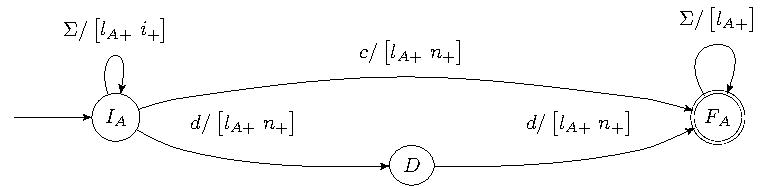
\includegraphics[width=\textwidth]{a}
    \caption{The automaton $A'$, whose Parikh registers count the length of the
    string accepted by the automaton (register $l_A$), the start offset of the
    substring ($i$) and length ($n$) of the substring matching
    $\Regex{c\RegexOr{}dd}$. Note the symbolic transitions in the starting and
    accepting states matching any symbol in the alphabet!}\label{fig:aut_a}
      %\Description[SHORT]{LONG}
  \end{subfigure}%
  \hfill%
  \begin{subfigure}[b]{\autscale\textwidth}
    \centering
    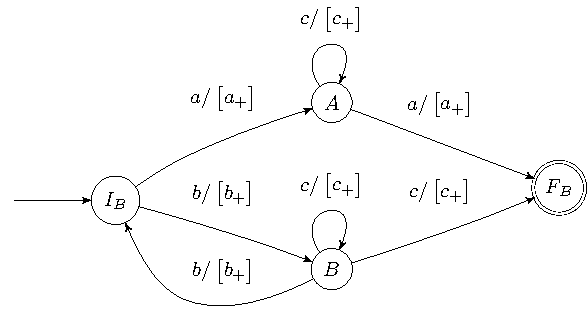
\includegraphics[width=\textwidth]{b}
    \caption{The automaton $B$, where the Parikh registers count the length of
    the string in register $l_B$.}\label{fig:aut_b}
      %\Description[SHORT]{LONG}
  \end{subfigure}
  \caption{The collection of automata we use as running
  examples, both derived from \cref{ex:string-constraints}.}\label{fig:examples}
\end{figure}

Intuitively, \cref{ex:string-constraints} is unsatisfiable. By inspecting the
automata, we realise that the path using $\Char{dd}$ in $\mathcal{A}'$ is unusable since
are no $\Char{d}$-labelled transitions in~$\mathcal{B}$. This means that $s_1 = \Char{c}$,
and thus $n = 1$. That means that \cref{const:more-inside-than-before} implies
that $i = 0$. However, no path through $B$ passes by a $\Char{c}$ without a
preceding character. Therefore, already
\cref{const:s1-in-c-dd,const:s1-in-c-dd,const:s1-substring,const:more-inside-than-before}
together are unsatisfiable.

%We will now proceed to show how we prove this using the three principles of
%\Calculus{}: problem-aware case splitting (sometimes called branching), lazy
%enforcement of connectivity constraints (essentially consisting of a constraint
%programming-style propagator), and lazy computation of products of automata.

An eager approach to finding the Parikh
image, as described in~\cite{generate-parikh-image}, would start by
computing the product $\mathcal{A}' \times \mathcal{B}$, translating it to a Presburger formula with
$i, n$, etc., as free variables, and then adding
\cref{const:more-inside-than-before,const:something-before-and-after} to the
resulting set of linear inequalitites. Scalability of this
construction is limited due to the size of the product automata to be computed,
and the complexity of the resulting Presburger formula.

\subsection{Solving the Parikh automata intersection problem using \Calculus{}}

We will now proceed to show how our calculus~\Calculus{} can lazily
prove the unsatisfiability of the running example. The calculus
interleaves several reasoning principles, which we will later
define precisely as calculus rules:
\begin{inparaenum}[(i)]
\item Similarly, as in \cite{generate-parikh-image}, we first describe
  each automaton as a flow network, counting how often each transition
  is taken in a run of the automaton. The flow constraints are an
  over-approximation of the possible accepting runs of an automaton.
\item We use a linear integer solver to simplify the flow constraints
  and prune away paths through the automata that are not feasible.
\item We use a tailor-made propagation algorithm to identify disconnected
  transitions of the automata that can never be taken and lazily add
  the corresponding constraints.
\item When propagation cannot infer further constraints, we use case
  splitting to subdivide the problem into smaller parts.
\item Once the constituent automata of a product have become
  sufficiently small, we compute the precise product automaton.
\end{inparaenum}

\subsubsection{Approximating paths through automata using flow analysis}\label{sec:a_1}

We associate each transition $\Transition$ of $\mathcal{A}'$ and $\mathcal{B}$ with a fresh
variable~$\TransitionVar_\Transition$ ranging over natural numbers (i.e.,
non-negative integers).
These variables represent how many times each
transition is taken. Hence, the final value for registers~$r_1, \ldots,
r_k$ of each automaton is the element-wise sum:
\begin{equation}\label{eq:counter-sums}
\begin{bmatrix} 
  r_1 \\
  \vdots\\
  r_k \\
\end{bmatrix} = \sum_\Transition \TransitionVar_\Transition \cdot 
  \IncrementVec_\Transition \text{ where $\IncrementVec_\Transition$ are the increments of transition $\Transition$}.
\end{equation}

We proceed by adding linear constraints requiring transition variables to
represent a flow through their automaton by adding linear constraints stating
that the number of incoming transitions is equal to the number of outgoing ones.
E.g., state $B$ of automaton~$\mathcal{B}$ would have the sum
%
\begin{equation}\label{eq:flow-eqs}
  \cancel{x_{\Tuple{B, \Char{c}, B}}} +
  x_{\Tuple{I_B, \Char{b}, B}} = \cancel{x_{\Tuple{B, \Char{c}, B}}}  +
  x_{\Tuple{B, \Char{c}, F_B}} + x_{\Tuple{B, \Char{b}, I_B}}
\end{equation}
%
where we let
$x_{\Tuple{q, l, q'}}$ refer to the integer variable associated with a
transition from state $q$ to state $q'$ with label $l$. The initial state
of the automaton receives an additional inflow of $1$, and accepting
states have an additional common outflow of $1$. Note that self-loops
cancels themselves out. Therefore, when a loop can become
unreachable, additional constraints are required to ensure consistency.

%\begin{figure}[tb]
%  \centering 
%  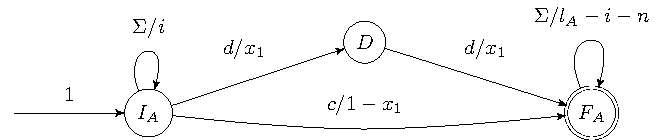
\includegraphics[width=0.6\textwidth]{a_1}
%  \caption{ $A'$ with its associated transition variables in symbolic form after
%  minimal elimination of variables using linear algebra. Note the incoming flow
%  of $1$ in the starting state and its balancing of the outgoing transitions!
%  }\label{fig:a_1}
%\end{figure}

\subsubsection{Arithmetic flow simplification}\label{sec:intuition:algebra}

We then use linear arithmetic reasoning on the register
equations~\eqref{eq:counter-sums} and flow
equations~\eqref{eq:flow-eqs} to simplify the counters associated
with transitions.
As an example, we start with $\mathcal{A}'$. Substituting back
solutions to the equations for $\mathcal{A}'$ to the automaton, we obtain the
automaton in \cref{fig:a_2}, where the notation~$a / t$ now denotes
a transition that accepts letter~$a$ and is taken~$t$ times.
In this case, the transitions of the automaton
can be specified purely in terms of the free
variables we care about representing:  the length of the accepted word ($l_A$), the
start of the substring ($i$), and the length of the substring ($n$).

\begin{figure}[tb]
  \centering 
  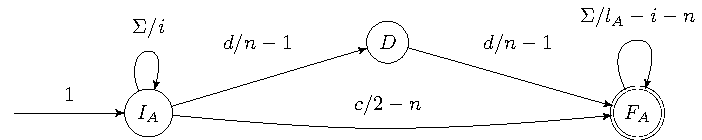
\includegraphics[width=0.6\textwidth]{a_2}
  \caption{ $\mathcal{A}'$ after even more simplification using linear algebra,
   with most transitions expressed
  in terms of $n$. Intuitively, this version captures the fact that $n$ is given
  by distributing the incoming flow of $1$ across the two outgoing transitions
  from $I_{A'}$, the initial state.}
  \label{fig:a_2}
\end{figure}

Having obtained this representation, we conclude that $1 < n \leq 2$
from
\cref{const:more-inside-than-before,const:something-before-and-after}. The
lower bound directly follows from
\cref{const:more-inside-than-before,const:something-before-and-after},
whereas the upper bound is obtained by the following reasoning. Since all
transition variables are non-negative integers (a transition cannot be
used a negative amount of times), $n \leq 2$ from the $I_A$ to $F_A$
transition. Therefore, it follows that $n=2$, which implies that the
$I_A$ to $F_A$ transition can never be used under these constraints
and that we must use the two $\Char{d}$-labelled transitions, both now
taken $n-1 =1$ times.
% This immediately implies that the problem is
%unsatisfiable, since we know this transition has no correspondance in
%automaton $B$.
%
Substituting the derived value of $n$ and applying similar
reasoning to automaton~$\mathcal{B}$, we arrive at the simplified
automata in \cref{fig:propagated}.

\begin{figure}[ht]
    \centering 
  \begin{subfigure}{0.42\textwidth}
    \centering
    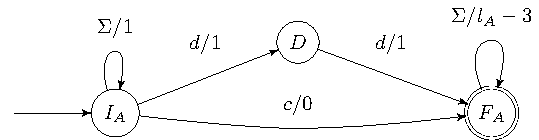
\includegraphics[width=\textwidth]{a_annotated}
    \vspace*{5ex}
    \caption{ $\mathcal{A}'$ with its associated transition variables in symbolic
    form.}\label{fig:aut_a_annotated}
      %\Description[SHORT]{LONG}
    \vspace*{1.9ex}
  \end{subfigure}\hfill%
  \begin{subfigure}{0.54\textwidth}
    \centering
    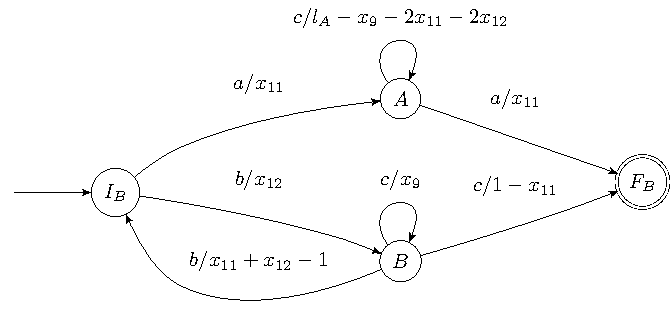
\includegraphics[width=\textwidth]{b_annotated}
    \caption{$\mathcal{B}$ with its associated transition variables in symbolic forms.
    The large number of implicitly existentially quantified
    variables~$x_i$ on
    transitions suggest that this automaton has a more complex structure
    with relation to its (free) target variable representing the string length
    than $\mathcal{A}'$. %The variables used here are fresh, and do not correspond to the
    % ones previously used.
  }\label{fig:aut_b_annotated}
      %\Description[SHORT]{LONG}
  \end{subfigure}
  \caption{The automata after arithmetic simplification.}\label{fig:propagated}
\end{figure}


Note that the per-automata length counting registers have been assigned the same
solver variable $l_A$. Since they have to be equal, either one can be used in
both automata through similar applications of equality elimination rules.

%\subsubsection{Connectivity reasoning}\label{sec:intuition:subsume}
%At this point we can conclude that none of the loops of $A'$ can become
%disconnected since they are at the initial and final states, both of which are
%reachable for any future assignments of the transition variables. This means
%that all valid counter assignments of $A'$ are described by
%\cref{eq:counter-sums} and the flow equations alone without the need for
%expensive connectivity constraints.

\subsubsection{Case Splitting and connectivity propagation}\label{sec:intuition:split}
We now have a choice of two paths through automaton $\mathcal{B}$; the
upper through state $A$ or the lower through state $B$. Since
arithmetic reasoning and propagation are not able to resolve this choice,
we perform a case split by selecting a transition variable that would disconnect
some strongly connected component of automaton $\mathcal{B}$, in this case the transition
from~$I_B$ to state $B$ guarded by variable~$x_{12}$.
 We split the reasoning into the cases $x_{12} > 0$ (transition used)
and $x_{12} = 0$ (transition unused). For presentation, we focus
on the latter case, as the former can be handled in a similar way.

In the case~$x_{12} = 0$, we can conclude
that the state~$B$ is now unreachable, which means that its outgoing transitions are now unusable. Propagation can
therefore infer the additional equations $x_9 = 0$ and $x_{11} = 1$.


\subsubsection{Computing products}\label{sec:intuition:materialise}
After discounting all transitions that can no longer be taken, we are
left with two (small) flat automata, and can compute their product with
relative ease. By putting off computing the product $\mathcal{B} \times \mathcal{A}'$ until after
performing linear reasoning, and using that to prune transitions, we
have computed a smaller product than we would have with an eager
approach. Computing the product, we will immediately notice that the
$\Char{d}$-labelled transition of automaton $\mathcal{A}'$ has no correspondence
in $\mathcal{B}$, leading to an empty product. We can close the proof goal and
backtrack, and we will eventually derive that the imposed constraints are
unsatisfiable by repeating the same process on the other branch.

%%% Local Variables:
%%% mode: latex
%%% TeX-master: "main"
%%% End:
